\chapter{引言}
\markboth{正文}{正文}

\setlength{\baselineskip}{20pt}

本章将主要介绍深度图像超分辨率重建的研究背景、研究现状、研究难点以及本文的研究内容与主要贡献。本章的组织结构如下:第一部分主要介绍深度图像超分辨率重建的研究背景以及该任务在实际应用中的研究意义和价值,第二部分将介绍深度图像超分辨率重建和单目深度估计的研究现状以及将两个任务统一于一个网络框架联合学习的主要难点,第三部分将介绍本文的主要研究内容和贡献,最后介绍论文的结构安排。

\section{研究背景与实际应用}

在理解场景时,人们不仅可以感知其外观(例如颜色,纹理等),还可以捕获深度信息以产生立体感。更好的场景理解可以促进自动驾驶 \cite{DBLP:conf/iros/KerlSC13},三维重建 \cite{DBLP:journals/pami/ImHCJJK19} 等依赖于高质量和高分辨率深度信息领域的研究。便携式消费级深度相机(如 Microsoft Kinect 和 Lidar)的出现和普及,为准确快速地获取场景深度提供了极大的便利。但是,由于当前深度相机成像能力的限制,深度图像的分辨率通常较低,无法与同场景的高分辨率彩色图像相匹配。面对诸多应用领域对高质量深度图像的需求 \cite{DBLP:journals/corr/abs-1907-06781, DBLP:journals/pami/GeLYT19, SilbermanHKF12},深度图像超分辨率重建技术作为解决方案获得了越来越多的关注。

深度图像超分辨率重建技术是指在不改变深度相机或深度传感器的前提下,通过算法恢复出相机或传感器截止频率以外的高频信息(图像的高频信息是指灰度变化快速的区域,例如物体边缘),同时改善成像时的模糊现象并有效抑制图像中的随机噪声,从而重建出高质量、高分辨率的深度图像。传统的基于滤波的方法 \cite{0001TT13,LuSMLD12} 和基于优化的方法 \cite{DBLP:conf/iccv/FerstlRRRB13, ParkKTBK11} 使用人工构造的滤波器或目标函数很难恢复出准确的高分辨率深度图像。近年来,随着深度学习的快速发展,许多研究已经表明了其在深度图像超分辨率重建任务上的有效性 \cite{HuiLT16, WenSLLF19}。基于卷积神经网络的深度图像超分辨率重建技术可以自动地从数据中学习更强的特征表示来重建高分辨率深度图像。

在实际应用中,高分辨率的彩色图像易于获得,且与深度图像具有很强的结构相似性,因而可以为深度图像超分辨率重建提供一些先验信息。这种利用彩色图像引导的深度图像超分辨率重建算法被称为颜色(或纹理图像)指导的深度图像超分辨率重建算法。现有的颜色指导的深度图像超分辨率重建算法通常需要一个额外的分支来从彩色图像中获取丰富的指导信息 \cite{LutioDWS19},然后利用它们来指导超分辨率重建分支对深度图像的特征提取。但是,彩色图像的结构并不总是与深度图像相一致。如 \ref{fig:1-1} 示,绿色矩形区域在彩色图像上具有复杂的纹理变化,但是由于目标内部的深度一致性,在对应的深度图像中该区域并没有表现出对应的纹理结构。因此,如果仅将从彩色图像提取的特征或边缘特征传递到超分辨率重建分支,就很容易造成诸如纹理复制和深度流失等问题。因此,探索如何有效地提取和利用高分辨率彩色图像蕴含的信息对于深度图像超分辨率重建任务非常重要。

\begin{figure}[!htbp]
\vspace{-0.8cm}  %调整图片与上文的垂直距离
	\centering
	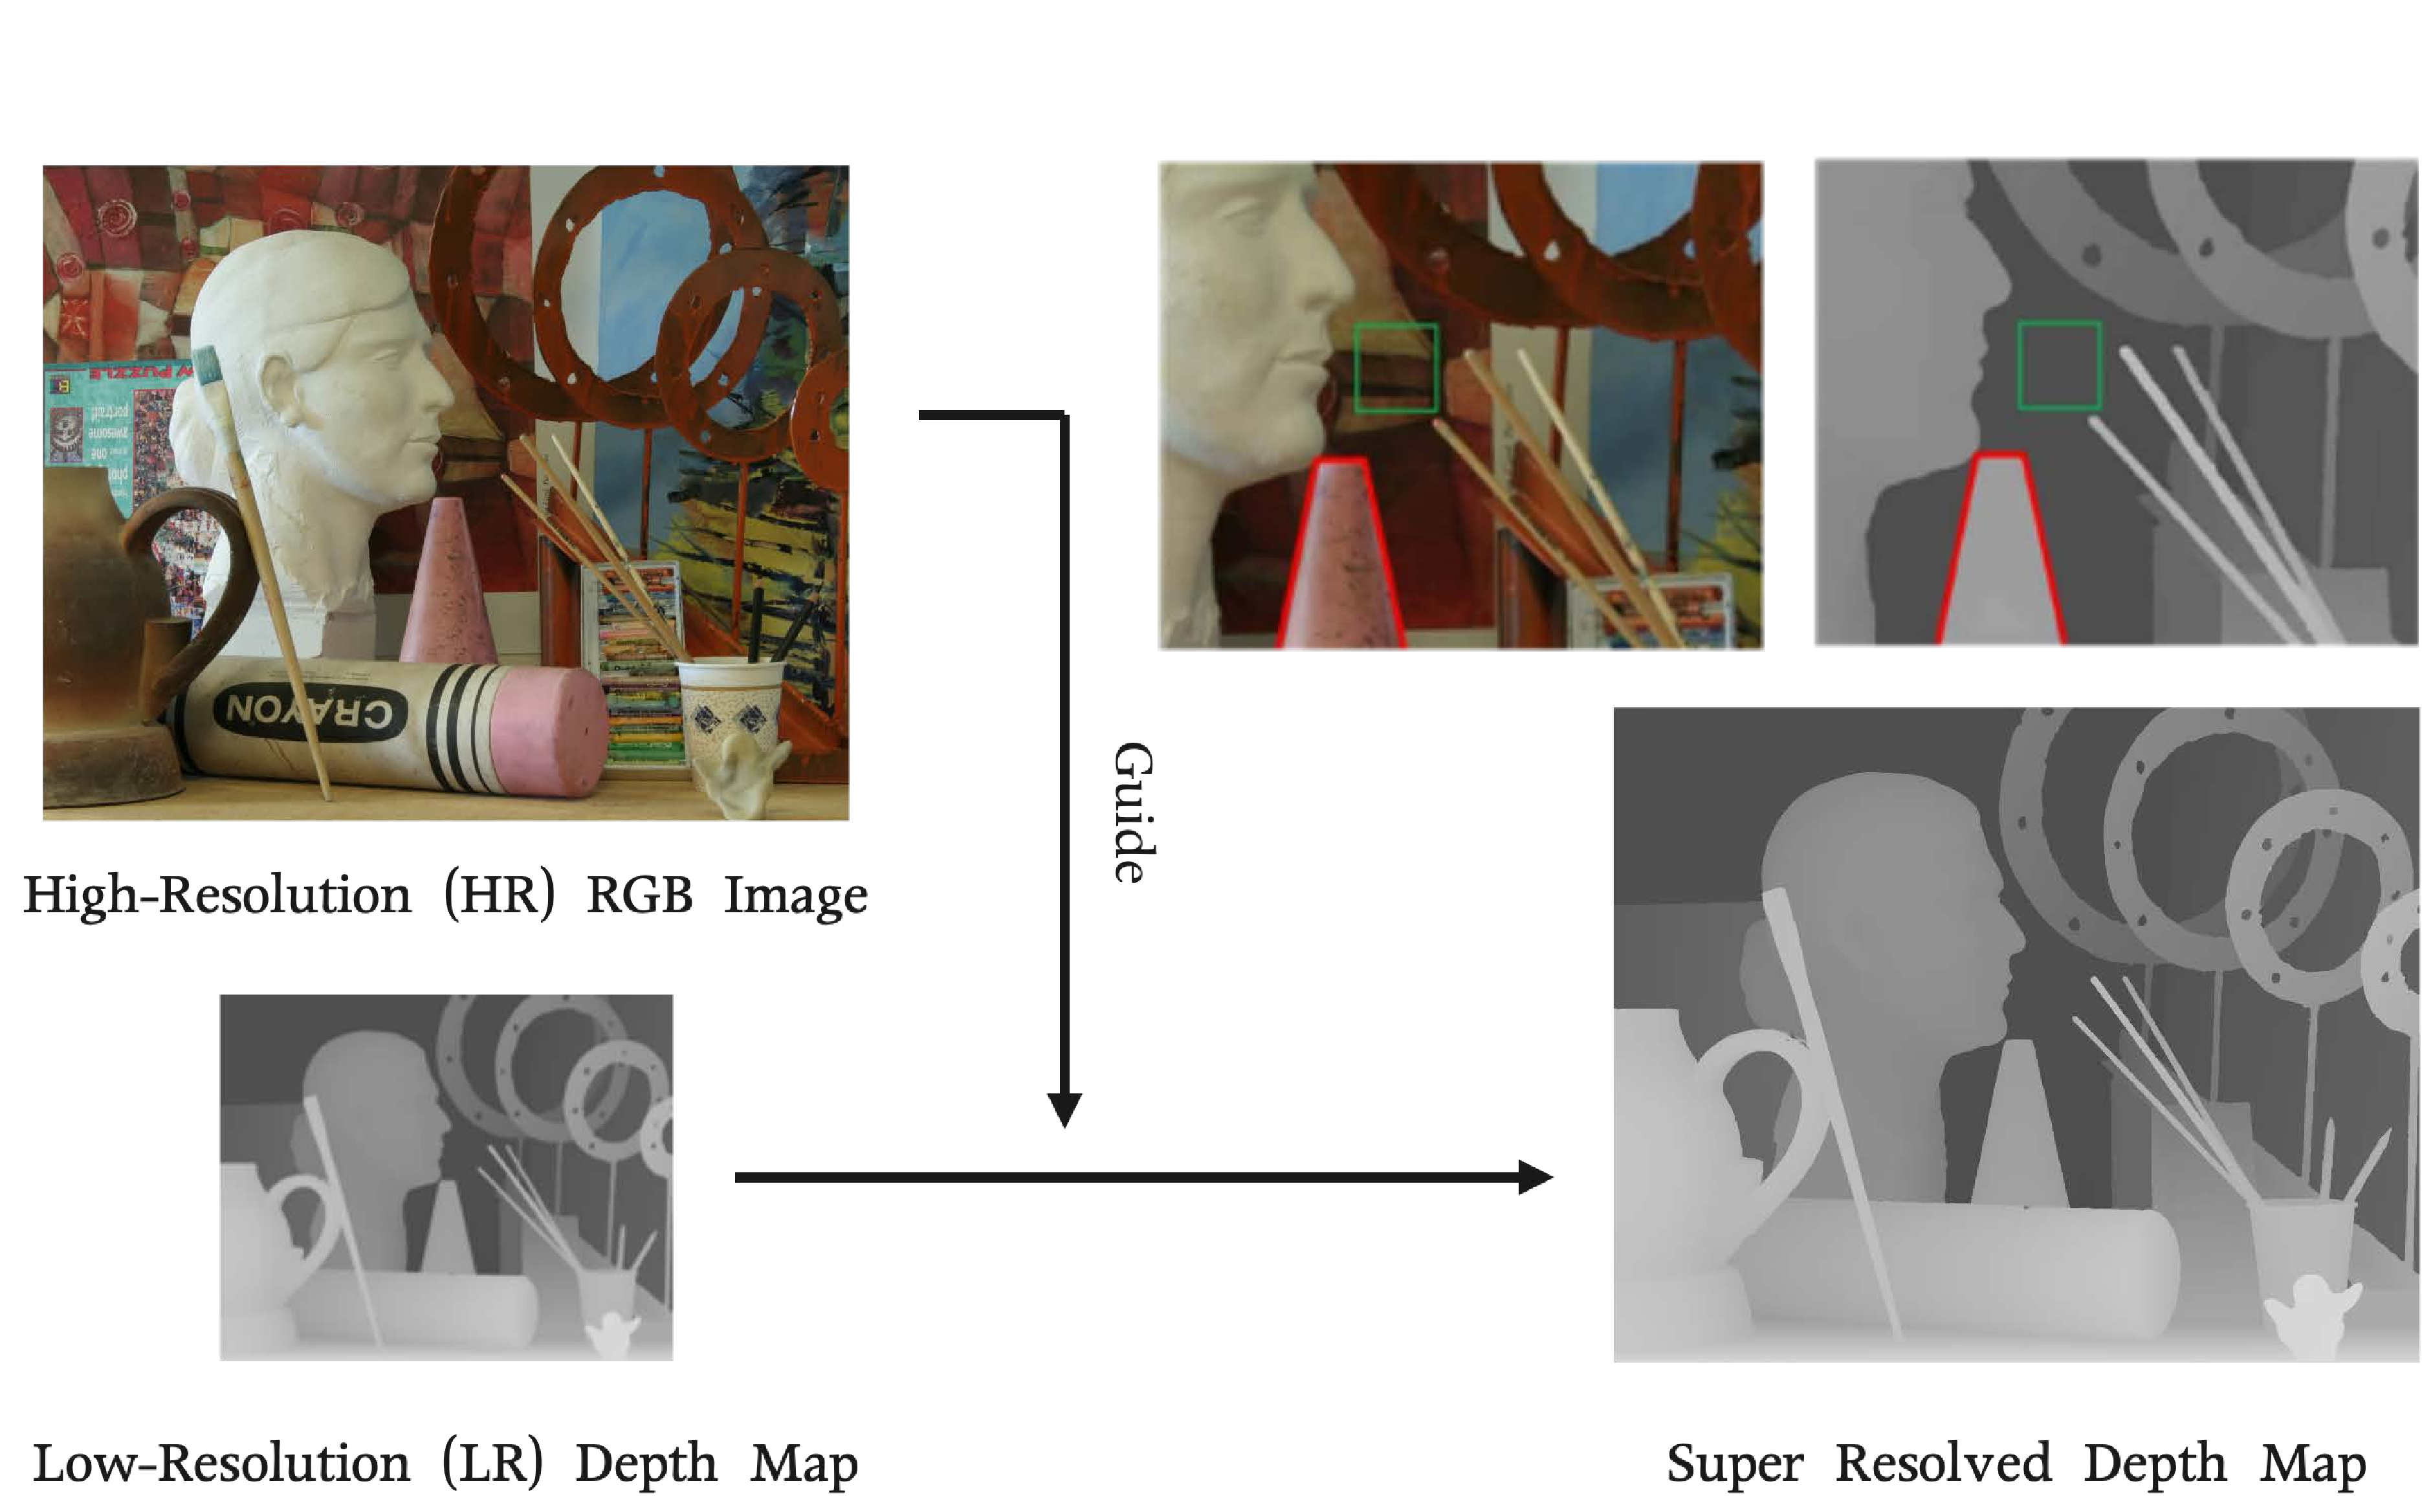
\includegraphics[scale=0.14]{figures/1}
	\caption{颜色引导的深度图像超分辨率重建示意图}
	\label{fig:1-1}
\end{figure}

为了寻找上述问题的解决方案,本文将目光聚焦在了另一个与深度图像有关的任务——单目深度估计。单目深度估计旨在将场景从光度表示映射到几何表示。具体而言,单目深度估计的输入是一幅彩色图像,而输出则是估计的深度图像。

单目深度估计与深度图像超分辨率重建两个任务是天然相关的:
\begin{enumerate}
	\item[(1)]	将两个任务嵌入联合学习的训练框架中,无需引入额外的监督标签(例如语义标签),即两个任务的训练数据集可以共享。
	\item[(2)] 由于单目深度估计可以在连续的训练和学习过程中实现从彩色图像到深度图像的跨模态信息转换,因而面向单目深度估计学习到的彩色图像特征更适合指导深度图像超分辨率重建。
\end{enumerate}

综上所述,深度图像超分辨率重建与单目深度估计的联合学习可以在不增加监督信息的情况下实现更好的颜色指导。

\section{研究现状及难点}

本部分将分别介绍深度图像超分辨率重建和单目深度估计的研究现状,并将详细分析将单目深度估计与深度图像超分辨率重建统一于联合学习框架的难点。

\subsection{深度图像超分辨率重建}

由于彩色图像和深度图像间的结构相似性,现有的许多方法都利用颜色信息指导低分辨率深度图像的重建。Zhao 等 \cite{DBLP:journals/corr/abs-1708-09105} 提出提出了彩色-深度条件生成对抗网络(Color-Depth Conditional Generative Adversarial Network, CDcGAN)来同时解决3D视频中的深度图像和彩色图像超分辨率重建问题,该网络考虑了同一场景下彩色图像和深度图像的结构相似性,采用彩色图像和深度图像的交互信息来相互促进彼此的性能。 Hui 等 \cite{HuiLT16} 设计了多尺度引导的卷积神经网络(Multi-Scale Guided convolutional network, MSG),将从彩色图像中提取的丰富层次特征用于改善深度图像超分辨率重建过程中图像的模糊现象。 Zuo 等 \cite{DBLP:journals/isci/ZuoFYSW19} 提出了彩色引导的深度图像增强残差稠密网络(Residual Dense Network for Guided Depth Enhancement, RDN-GDE),将多尺度残差与稠密连接相结合以逐步增强低分辨率的深度图像。 Ye 等 \cite{DBLP:journals/tip/YeSWYXLL20} 提出了渐进的多分支聚合网络(Progressive Multi-Branch Aggregation network, PMBA), 通过重建分支和引导分支融合的方式逐步优化反卷积得到的高分辨率深度图像。 Guo 等 \cite{DBLP:journals/tip/GuoLGCFH19} 提出了层次特征驱动的深度图像超分辨率重建残差网络 DepthSR-Net, 利用 U-Net 结构对插值后的深度图像进行编码,并在解码过程中与相应尺度的彩色特征进行融合。

\subsection{单目深度估计}

单目深度估计是一个典型的不适定逆问题,这是由于其将在信息不足以完全指定解决方案的情况下尝试恢复一些未知数。与基于左右视图的深度估计任务相比,单目深度估计具有更加广阔的实际应用前景,但目前单目深度估计的性能仍然非常有限。Eigen 等 \cite{DBLP:conf/nips/EigenPF14} 设计了一个包含对场景全局的粗估计和局部区域的精估计两个尺度的卷积神经网络,开创了深度学习在单目深度估计领域的先河。Laina等 \cite{DBLP:conf/3dim/LainaRBTN16} 使用了更深的残差网络并通过小卷积进行上采样,从而提升了单目深度估计的效率。Cao等 \cite{DBLP:journals/tcsv/CaoWS18} 将原始的连续深度离散为固定数量的深度范围,进而将单目深度估计从回归任务转换为分类任务,观察到了明显的性能提升。

\subsection{面向深度图像的多任务联合学习}

多任务学习的目的是通过相关任务联合以提升特定任务的性能,最简单的联合方法是通过损失函数将两个或多个任务组合在一起。但由于在网络设计中缺乏交互性,这通常不是最佳的策略。目前,许多与深度图像处理有关的任务都采用了多任务学习策略。Zhang 等 \cite{DBLP:conf/eccv/ZhangCXJLY18} 提出的联合任务递归学习(Joint Task-Recursive Learning, TRL)框架将问题序列化为任务交替的时间序列来递归地优化语义分割和单目深度估计任务的结果。这类方法仅仅通过网络和损失约束的设计来驱动两个任务的联合学习,而没有明确地探究任务之间存在的约束。He等 \cite{DBLP:journals/corr/abs-2101-07422} 基于两个任务的几何约束提出联合语义分割的单目深度估计网络(Semantic Object Segmentation and Depth Estimation Network, SOSD-Net)这一工作明确探究了多任务学习中任务之间的关联性,但单目深度估计和语义分割的相关性仍然较弱。此外,相对于单目深度估计而言,这些方法在训练时需要引入额外的标签(如语义标签)。Sun 等 \cite{Sun2021cvpr} 提出了一种通过单目深度估计在训练过程中帮助深度图像超分辨率重建更好地理解场景结构的知识蒸馏方法,从而证明了单目深度估计在改善深度图像超分辨率重建性能方面的有效性。但其通过比较训练过程中两个任务的平均像素误差来确定两个任务交互方向的方法,并没有明确地探究深度图像超分辨率重建与单目深度估计的相关性。

综上,联合单目深度估计的深度图像超分辨率重建的研究难点在于探究两个任务的关联性并设计合理的交互方式,尤其是探究如何将深度估计学习到的“知识”通过多任务学习的模式帮助低分辨率的深度图像进行超分辨率重建,从而达到更好的重建效果。


\section{本文主要工作}

受上述分析的驱动,本文提出了深度图像超分辨率重建和单目深度估计的联合学习网络(BridgeNet),关注于通过有效地桥接两个任务以实现更好的深度图像超分辨率重建。本文基于编码器-解码器(Encoder-Decoder)结构分别为单目深度估计和深度图像超分辨率重建任务设计了两个子网络,即深度图像超分辨率重建子网络(DSRNet)和单目深度估计子网络(MDENet),它们以多任务学习的模式协同工作。此外,本文还分别在编码器和解码器中设计了两个不同的桥接器(Bridge)以实现两个子网络的差异化引导。具体而言,单目深度估计子网络的编码器从彩色图像中学习面向深度图像的多级特征,这样的彩色特征更适用于指导深度图像的超分辨率重建。因此,本文提出了一个高频注意力桥(HABdg),将单目深度估计学习到的高频信息用于指导深度图像超分辨率重建。 单目深度估计子网络和深度图像超分辨率重建子网络的特征解码器用于进一步提取面向任务的特征,以进行深度估计和深度图像超分辨率重建。由于单目深度估计存在的尺度模糊性,单目深度估计相较于深度图像的超分辨率重建更难达到良好的性能。因此,遵循简单任务指导困难任务的原则,本文提出了内容引导桥(CGBdg),旨在使深度图像超分辨率重建子网络在深度特征空间为单目深度估计子网络提供内容引导。除了在模型设计层面上关联这两个任务外,本文还在损失函数方面对其进行约束,以期两个子网络可以相互促进。

综上所述,本文主要贡献如下:
\begin{enumerate}[leftmargin=55bp]
\item[(1)]	本文在联合学习网络中将深度图像超分辨率重建任务和单目深度估计任务相关联,以提升深度图像超分辨率重建的性能。本文提出的联合学习网络包括深度图像超分辨率重建子网络(DSRNet)和单目深度估计子网络(MDENet),以及两个用于联合学习的桥接器,即高频注意力桥(HABdg)和内容引导桥(CGBdg)。本文的整个网络结构具有高度的可移植性,可以为关联深度图像超分辨率重建和单目深度估计任务提供范例。此外,与其他多任务学习不同,本文用于联合学习的两个任务不需要引入其他的监督信息。  
\item[(2)]	 特征编码阶段中的高频注意力桥(HABdg)将从单目深度估计子网络学习到的彩色高频信息传输到深度图像超分辨率重建子网络,从而可以提供更接近深度模态的颜色指导信息。遵循简单任务指导困难任务的原则,本文在特征解码阶段切换了两个任务的指导角色,并提出了内容引导桥(CGBdg),从而可以让深度图像超分辨率重建子网络在深度特征空间为单目深度估计子网络提供内容引导。
\item[(3)]	在不引入其他监督信息的情况下,本文的方法在多个公开基准数据集上均达到了具有竞争力的性能。 
\end{enumerate}


\section{结构安排}

本文一共分为五章,每一章节的内容安排如下:

第一章为引言,以深度图像超分辨率重建的研究背景和现实意义、颜色引导的深度图像超分辨率重建存在的问题、单目深度估计与深度图像超分辨率重建颜色分支的相似性为脉络层层递进,进而引出本文在多任务学习模式下将深度估计和深度图像超分辨率重建相关联的研究内容,接着分别介绍了两个任务的研究现状以及将他们统一于一个网络框架联合学习的关键难点,最后对论文的结构组织进行介绍。

第二章为相关技术和方法介绍,主要介绍了与本文研究相关的技术和方法,即联合单目深度估计的深度图像超分辨率重建网络的基石。

第三章为算法实现,详细地介绍了单目深度估计和深度图像超分辨率重建联合学习网络的架构设计,包括深度图像超分辨率重建子网络,单目深度估计子网络以及高频注意力桥和内容引导桥。

第四章为实验测试与分析,介绍了本文了采用的公开基准数据集和评估指标,然后对比分析了本文设计的网络在所选公开基准数据集上进行训练和测试的性能表现,以及与其他最新的深度图像超分辨率重建网络性能的对比。此外,通过消融实验验证了不同设计对网络性能的影响。

第五章为结论,对本文的工作进行总结,囊括了本文的主要贡献,并概述了未来工作的研究方向。


\section{本章小结}

本章层层递进地介绍了深度图像超分辨率重建的研究背景和意义,然后从颜色引导的深度图像超分辨率重建存在的问题出发,阐明了联合单目深度估计与深度图像超分辨率重建联合学习算法的研究动机,进而分别介绍了两个任务的研究现状以及探究两个任务的关联性在是设计两个任务联合学习网络的重点和难点,然后对本文的主要贡献进行了详细介绍。
